\section{Results}
\subsection{RQ1--RQ2: structure and complementary support}
There are 75 structural rejects (12.48\%): five of 200 Abalone19, six of 201 Ecoli4 and 64 of 200 page-blocks0. Fifteen records lack class, one lacks features and 64 have fractional-integer fields; categories overlap. Twenty-six violate multiple fields. No unsupported nominal value or invalid numerical primitive appears in this population.

Local/global Spearman correlations are $.908$, $.488$ and $.621$ for Abalone19, Ecoli4 and page-blocks0, with respectively 14, 30 and two tail-disagreement cases. The scores are related but do not identify identical concerns. Combined admission yields 170, 162 and 119 provisional passes, versus 195, 195 and 136 with structure only. Existing local/global, $k$/shrinkage and cutoff sensitivities are reused unchanged. These results establish distinct statistical information and eligibility, not semantic-error detection performance.

\subsection{RQ3: matched-budget ablations}
\begingroup\scriptsize\begin{longtable}{lrrrrrrr}
\caption{Consolidated historical ablations. Q denotes unchanged quality-coverage selection. Random rows average five seeds; complete per-seed data accompany the paper. F1 is logistic pure TSTR; -- means unavailable.}\label{tab:ablations}\\
\toprule
Dataset & Method & Pool & $n$ & Coverage & Exact & Near & F1 \\
\midrule\endfirsthead
\toprule
Dataset & Method & Pool & $n$ & Coverage & Exact & Near & F1 \\
\midrule\endhead
Abalone19 & Raw labeled random & 195 & 56 & 0.799 & 0.171 & 0.443 & 0.029 \\
 & Schema random & 195 & 56 & 0.799 & 0.171 & 0.443 & 0.029 \\
 & Admitted random & 170 & 56 & 0.833 & 0.236 & 0.493 & 0.022 \\
 & Structure + Q selection & 195 & 56 & 0.951 & 0.000 & 0.000 & 0.030 \\
 & Structure/local + Q & 177 & 56 & 0.950 & 0.000 & 0.000 & 0.031 \\
 & Structure/global + Q & 177 & 56 & 0.948 & 0.000 & 0.000 & 0.031 \\
 & Structure/local/global + Q & 170 & 56 & 0.948 & 0.000 & 0.000 & 0.031 \\
 & Admitted source order & 170 & 56 & 0.622 & 0.357 & 0.625 & -- \\
 & Admitted farthest first & 170 & 56 & 0.940 & 0.000 & 0.000 & 0.035 \\
 & Admitted coverage greedy & 170 & 56 & 0.948 & 0.107 & 0.268 & 0.030 \\
 & Repair pool + Q & 170 & 56 & 0.948 & 0.000 & 0.000 & 0.031 \\
Ecoli4 & Raw labeled random & 195 & 70 & 0.422 & 0.097 & 0.180 & 0.253 \\
 & Schema random & 195 & 70 & 0.422 & 0.097 & 0.180 & 0.253 \\
 & Admitted random & 162 & 70 & 0.439 & 0.117 & 0.197 & 0.217 \\
 & Structure + Q selection & 195 & 70 & 0.509 & 0.000 & 0.000 & 0.216 \\
 & Structure/local + Q & 175 & 70 & 0.509 & 0.000 & 0.000 & 0.195 \\
 & Structure/global + Q & 177 & 70 & 0.506 & 0.000 & 0.000 & 0.229 \\
 & Structure/local/global + Q & 162 & 70 & 0.506 & 0.000 & 0.000 & 0.205 \\
 & Admitted source order & 162 & 70 & 0.416 & 0.200 & 0.386 & -- \\
 & Admitted farthest first & 162 & 70 & 0.468 & 0.000 & 0.000 & 0.200 \\
 & Admitted coverage greedy & 162 & 70 & 0.506 & 0.114 & 0.243 & 0.108 \\
 & Repair pool + Q & 162 & 70 & 0.506 & 0.000 & 0.000 & 0.205 \\
page-blocks0 & Raw labeled random & 195 & 49 & 0.905 & 0.061 & 0.559 & 0.390 \\
 & Schema random & 136 & 49 & 0.889 & 0.069 & 0.559 & 0.477 \\
 & Admitted random & 119 & 49 & 0.914 & 0.082 & 0.702 & 0.535 \\
 & Structure + Q selection & 136 & 49 & 0.934 & 0.000 & 0.286 & 0.202 \\
 & Structure/local + Q & 120 & 49 & 0.932 & 0.000 & 0.327 & 0.446 \\
 & Structure/global + Q & 120 & 49 & 0.934 & 0.000 & 0.327 & 0.448 \\
 & Structure/local/global + Q & 119 & 49 & 0.932 & 0.000 & 0.327 & 0.446 \\
 & Admitted source order & 119 & 49 & 0.914 & 0.265 & 0.592 & -- \\
 & Admitted farthest first & 119 & 49 & 0.932 & 0.000 & 0.000 & 0.550 \\
 & Admitted coverage greedy & 119 & 49 & 0.932 & 0.163 & 0.449 & 0.627 \\
 & Repair pool + Q & 168 & 49 & 0.937 & 0.000 & 0.102 & 0.342 \\
\bottomrule\end{longtable}
\endgroup
Table~\ref{tab:ablations} consolidates structure, local/global admission, selection and repair. Every construction reaches its declared budget. Random rows average all five seeds; individual results and variability accompany the paper. Raw-labeled controls remove class/feature-incomplete records explicitly.

Quality-coverage increases distinct-feature TRAIN coverage over source order from $.6225$ to $.9479$ on Abalone19 and $.4164$ to $.5056$ on Ecoli4, with zero exact/near redundancy on both. Farthest-first removes redundancy but has lower Ecoli4 coverage ($.4684$). Coverage-greedy reaches $.5056$ with exact duplication $.1143$. These metrics distinguish different selection behavior. Combined eligibility, quotas and coverage objectives prevent interpreting this comparison as the isolated causal effect of an evidence score.
Structure-only admission followed by the same quality selector slightly exceeds full-admission coverage on Abalone19 ($.951$ versus $.948$) and Ecoli4 ($.509$ versus $.506$). On page-blocks0, full admission instead improves logistic pure-TSTR F1 over structure only ($.446$ versus $.202$). Additional evidence therefore changes outcomes without producing monotonic gains across datasets or metrics.

\begin{figure}[htbp]\centering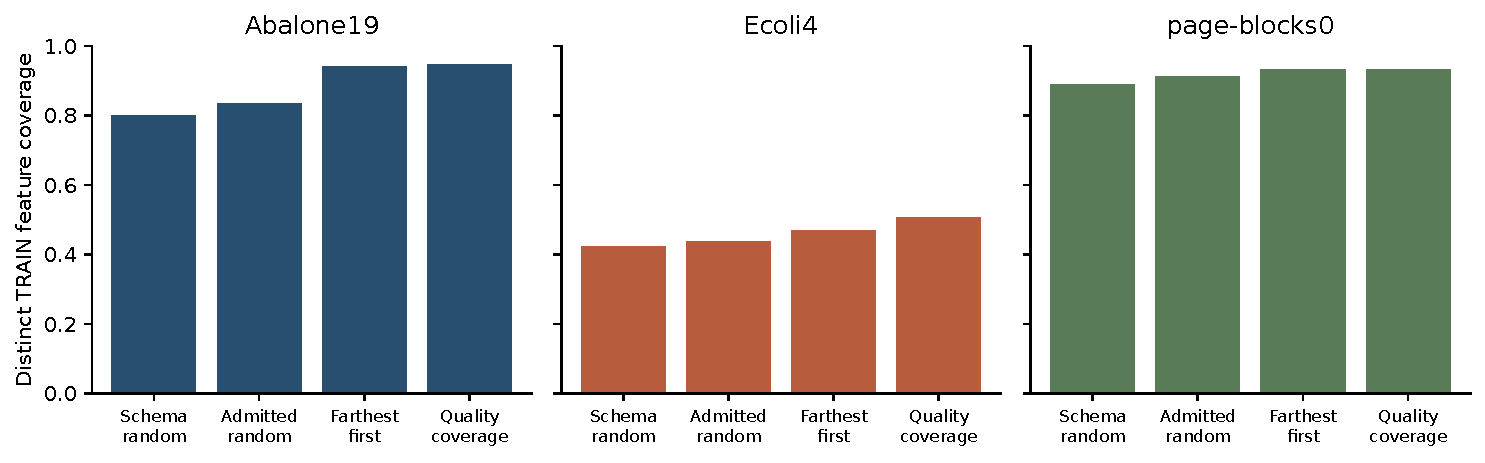
\includegraphics[width=\linewidth]{figures/coverage.pdf}
\caption{Historical fixed-budget distinct-feature TRAIN coverage. Random bars average five selection seeds; admitted selectors share the same pool.}\label{fig:coverage}\end{figure}

\subsection{RQ4: bounded repair}
All 54 eligible repairs become structurally compliant; 21 rejected records are ineligible. Repairs edit 73 fields: 39 records require one edit, eleven two and four three. Absolute changes range $.1$--$.5$, mean $.3119$. Five fractional-integer records also lack class and five require over three edits; neither group is repaired. Eleven further ineligible records belong to Abalone19/Ecoli4.

Under unchanged admission, 49 derived versions provisionally pass and five require review. The page-blocks0 admitted pool grows 119 to 168. At budget 49, quality-coverage selects 16 derived records: distinct-feature coverage rises $.9324$ to $.9370$, near duplication falls $.3265$ to $.1020$ and exact duplication remains zero. Source-order coverage slightly declines; other datasets are unchanged. Expanded pools therefore have method-dependent effects.

\subsection{RQ5: utility and external comparators}
All 138 historical utility rows reproduce within $10^{-12}$, including 24 unavailable cases. The expanded study contains 894 utility rows: 678 successful and 216 explicitly unavailable, without execution failures or budget shortfalls. Complete files retain both classifiers, regimes, class counts, confusion counts and metrics. Eighteen additional method/type incompatibilities are listed separately.

\begingroup\small\begin{longtable}{lrrrrrr}
\caption{Historical external training baselines. ROS and SMOTE/NC append b minority rows. LR: logistic regression; RF: random forest. These differ from candidate curation.}\label{tab:external}\\
\toprule
Dataset / method & Model & $+n$ & F1 & AP & BA & MCC \\
\midrule\endfirsthead
\toprule
Dataset / method & Model & $+n$ & F1 & AP & BA & MCC \\
\midrule\endhead
Abalone19 / Real & LR & 0 & 0.000 & 0.026 & 0.500 & 0.000 \\
Abalone19 / Real & RF & 0 & 0.000 & 0.023 & 0.500 & 0.000 \\
Abalone19 / Weighted LR & LR & 0 & 0.054 & 0.038 & 0.873 & 0.144 \\
Abalone19 / ROS+b & LR & 56 & 0.000 & 0.031 & 0.500 & 0.000 \\
Abalone19 / ROS+b & RF & 56 & 0.000 & 0.031 & 0.500 & 0.000 \\
Abalone19 / SMOTENC+b & LR & 56 & 0.000 & 0.014 & 0.499 & -0.003 \\
Abalone19 / SMOTENC+b & RF & 56 & 0.000 & 0.020 & 0.499 & -0.003 \\
Ecoli4 / Real & LR & 0 & 1.000 & 1.000 & 1.000 & 1.000 \\
Ecoli4 / Real & RF & 0 & 0.667 & 1.000 & 0.750 & 0.696 \\
Ecoli4 / Weighted LR & LR & 0 & 0.800 & 1.000 & 0.984 & 0.803 \\
Ecoli4 / ROS+b & LR & 70 & 1.000 & 1.000 & 1.000 & 1.000 \\
Ecoli4 / ROS+b & RF & 70 & 0.857 & 1.000 & 0.875 & 0.859 \\
Ecoli4 / SMOTE+b & LR & 70 & 1.000 & 1.000 & 1.000 & 1.000 \\
Ecoli4 / SMOTE+b & RF & 70 & 0.857 & 1.000 & 0.875 & 0.859 \\
page-blocks0 / Real & LR & 0 & 0.715 & 0.746 & 0.802 & 0.699 \\
page-blocks0 / Real & RF & 0 & 0.869 & 0.921 & 0.911 & 0.856 \\
page-blocks0 / Weighted LR & LR & 0 & 0.721 & 0.768 & 0.903 & 0.696 \\
page-blocks0 / ROS+b & LR & 49 & 0.728 & 0.746 & 0.811 & 0.712 \\
page-blocks0 / ROS+b & RF & 49 & 0.864 & 0.920 & 0.906 & 0.851 \\
page-blocks0 / SMOTE+b & LR & 49 & 0.728 & 0.758 & 0.811 & 0.712 \\
page-blocks0 / SMOTE+b & RF & 49 & 0.869 & 0.916 & 0.911 & 0.856 \\
\bottomrule\end{longtable}
\endgroup
External training baselines retain actual training populations and generated structural-compliance counts. Standard SMOTE's page-blocks0 outputs are not integer-coerced. Class weighting changes the training objective without generating records. These interventions are not matched candidate-curation alternatives.
In the historical page-blocks0 SMOTE baseline, 46 of 49 generated rows fail the integer structural contract; all remain computationally evaluable numerical augmentation records, and this incompatibility is explicit rather than repaired silently.

For historical page-blocks0 logistic pure TSTR, repair-pool expansion changes F1 from $.4464$ to $.3421$, while AP changes $.5552$ to $.5716$. Hybrid F1 stays $.7150$. This negative result accompanies improved coverage and near redundancy: geometric gains do not ensure utility gains.

\subsection{RQ6: conditional uncertainty and fresh-split stability}
\begingroup\scriptsize\setlength{\tabcolsep}{2pt}\begin{longtable}{lrrrrr}
\caption{Conditional 95\% bootstrap intervals (2,000 stratified paired resamples). Q: quality-coverage pure TSTR; Real: TRTR. Degenerate MCC intervals are unavailable; all valid counts are saved.}\label{tab:bootstrap}\\
\toprule
Dataset / method & Model & F1 [CI] & AP [CI] & BA [CI] & MCC [CI] \\
\midrule\endfirsthead
\toprule
Dataset / method & Model & F1 [CI] & AP [CI] & BA [CI] & MCC [CI] \\
\midrule\endhead
Abalone19 / Real & LR & 0.000 [0.000, 0.000] & 0.026 [0.022, 0.044] & 0.500 [0.500, 0.500] & 0.000 [--, --] \\
Abalone19 / Real & RF & 0.000 [0.000, 0.000] & 0.023 [0.012, 0.047] & 0.500 [0.500, 0.500] & 0.000 [--, --] \\
Abalone19 / Q & LR & 0.031 [0.029, 0.034] & 0.019 [0.012, 0.068] & 0.775 [0.758, 0.791] & 0.093 [0.087, 0.100] \\
Abalone19 / Q & RF & 0.030 [0.018, 0.039] & 0.021 [0.011, 0.046] & 0.724 [0.553, 0.820] & 0.078 [0.018, 0.112] \\
Abalone19 / Q repair & LR & 0.031 [0.029, 0.034] & 0.019 [0.012, 0.068] & 0.775 [0.758, 0.791] & 0.093 [0.087, 0.100] \\
Abalone19 / Q repair & RF & 0.030 [0.018, 0.039] & 0.021 [0.011, 0.046] & 0.724 [0.553, 0.820] & 0.078 [0.018, 0.112] \\
Ecoli4 / Real & LR & 1.000 [1.000, 1.000] & 1.000 [1.000, 1.000] & 1.000 [1.000, 1.000] & 1.000 [1.000, 1.000] \\
Ecoli4 / Real & RF & 0.667 [0.000, 1.000] & 1.000 [1.000, 1.000] & 0.750 [0.500, 1.000] & 0.696 [0.489, 1.000] \\
Ecoli4 / Q & LR & 0.205 [0.170, 0.258] & 0.135 [0.109, 0.267] & 0.754 [0.690, 0.817] & 0.241 [0.188, 0.307] \\
Ecoli4 / Q & RF & 0.296 [0.235, 0.400] & 0.633 [0.348, 1.000] & 0.849 [0.794, 0.905] & 0.349 [0.280, 0.450] \\
Ecoli4 / Q repair & LR & 0.205 [0.170, 0.258] & 0.135 [0.109, 0.267] & 0.754 [0.690, 0.817] & 0.241 [0.188, 0.307] \\
Ecoli4 / Q repair & RF & 0.296 [0.235, 0.400] & 0.633 [0.348, 1.000] & 0.849 [0.794, 0.905] & 0.349 [0.280, 0.450] \\
page-blocks0 / Real & LR & 0.715 [0.637, 0.783] & 0.746 [0.663, 0.832] & 0.802 [0.754, 0.845] & 0.699 [0.619, 0.769] \\
page-blocks0 / Real & RF & 0.869 [0.819, 0.914] & 0.921 [0.868, 0.965] & 0.911 [0.872, 0.944] & 0.856 [0.802, 0.904] \\
page-blocks0 / Q & LR & 0.446 [0.395, 0.500] & 0.555 [0.458, 0.656] & 0.759 [0.715, 0.804] & 0.389 [0.325, 0.456] \\
page-blocks0 / Q & RF & 0.342 [0.308, 0.377] & 0.447 [0.368, 0.534] & 0.727 [0.685, 0.768] & 0.288 [0.234, 0.342] \\
page-blocks0 / Q repair & LR & 0.342 [0.303, 0.383] & 0.572 [0.482, 0.676] & 0.713 [0.669, 0.758] & 0.278 [0.222, 0.337] \\
page-blocks0 / Q repair & RF & 0.316 [0.283, 0.350] & 0.474 [0.391, 0.572] & 0.704 [0.661, 0.748] & 0.254 [0.200, 0.309] \\
\bottomrule\end{longtable}
\endgroup
The 216 endpoint and 168 paired-difference intervals derive from saved predictions. Page-blocks0 logistic repair-minus-original F1 is approximately $-.1043$, with conditional interval $[-.1350,-.0739]$; AP difference is $.0165$, interval $[-.0071,.0493]$. F1 decreases consistently under this conditional resampling design, while AP direction is less stable. These remain descriptive intervals on reused historical TEST.

Ecoli4 logistic TRTR predicts perfectly on only four positive and 63 negative TEST records, yielding conditional F1 interval $[1,1]$. Its Wilson positive-recall interval is approximately $[.510,1]$. Resampling perfect observed predictions cannot establish universal performance. Abalone19 has only six positive TEST examples; resampling adds no independent positive observations.

\begingroup\scriptsize\begin{longtable}{lrrrrr}
\caption{Offline replication: five repeated stratified holdouts, logistic regression, mean $\pm$ sample SD. Real and weighted are TRTR; other methods are hybrid minority augmentation. No historical candidates are reused.}\label{tab:repeated}\\
\toprule
Dataset / method & $k$ & F1 & AP & BA & MCC \\
\midrule\endfirsthead
\toprule
Dataset / method & $k$ & F1 & AP & BA & MCC \\
\midrule\endhead
Abalone19 / Weighted LR & 5 & 0.051 $\pm$ 0.009 & 0.045 $\pm$ 0.014 & 0.779 $\pm$ 0.071 & 0.116 $\pm$ 0.028 \\
Abalone19 / Real & 5 & 0.000 $\pm$ 0.000 & 0.042 $\pm$ 0.015 & 0.500 $\pm$ 0.000 & 0.000 $\pm$ 0.000 \\
Abalone19 / ROS+b & 5 & 0.000 $\pm$ 0.000 & 0.040 $\pm$ 0.014 & 0.500 $\pm$ 0.001 & -0.002 $\pm$ 0.002 \\
Abalone19 / SMOTENC+b & 5 & 0.000 $\pm$ 0.000 & 0.041 $\pm$ 0.013 & 0.500 $\pm$ 0.000 & -0.002 $\pm$ 0.002 \\
Abalone19 / Curated Q & 5 & 0.000 $\pm$ 0.000 & 0.044 $\pm$ 0.011 & 0.500 $\pm$ 0.001 & -0.002 $\pm$ 0.002 \\
Abalone19 / Admitted random & 5 & 0.000 $\pm$ 0.000 & 0.047 $\pm$ 0.016 & 0.500 $\pm$ 0.000 & -0.001 $\pm$ 0.002 \\
Abalone19 / Schema random & 5 & 0.000 $\pm$ 0.000 & 0.041 $\pm$ 0.012 & 0.500 $\pm$ 0.000 & -0.002 $\pm$ 0.002 \\
Ecoli4 / Weighted LR & 5 & 0.695 $\pm$ 0.117 & 0.923 $\pm$ 0.053 & 0.928 $\pm$ 0.074 & 0.692 $\pm$ 0.127 \\
Ecoli4 / Real & 5 & 0.848 $\pm$ 0.119 & 0.944 $\pm$ 0.058 & 0.875 $\pm$ 0.088 & 0.855 $\pm$ 0.108 \\
Ecoli4 / ROS+b & 5 & 0.745 $\pm$ 0.177 & 0.908 $\pm$ 0.055 & 0.865 $\pm$ 0.089 & 0.744 $\pm$ 0.182 \\
Ecoli4 / SMOTE+b & 5 & 0.758 $\pm$ 0.166 & 0.944 $\pm$ 0.058 & 0.867 $\pm$ 0.089 & 0.757 $\pm$ 0.170 \\
Ecoli4 / Curated Q & 5 & 0.758 $\pm$ 0.166 & 0.934 $\pm$ 0.050 & 0.867 $\pm$ 0.089 & 0.757 $\pm$ 0.170 \\
Ecoli4 / Admitted random & 5 & 0.758 $\pm$ 0.166 & 0.934 $\pm$ 0.050 & 0.867 $\pm$ 0.089 & 0.757 $\pm$ 0.170 \\
Ecoli4 / Schema random & 5 & 0.758 $\pm$ 0.166 & 0.944 $\pm$ 0.058 & 0.867 $\pm$ 0.089 & 0.757 $\pm$ 0.170 \\
page-blocks0 / Weighted LR & 5 & 0.708 $\pm$ 0.029 & 0.788 $\pm$ 0.024 & 0.913 $\pm$ 0.013 & 0.687 $\pm$ 0.031 \\
page-blocks0 / Real & 5 & 0.728 $\pm$ 0.026 & 0.800 $\pm$ 0.019 & 0.819 $\pm$ 0.025 & 0.709 $\pm$ 0.025 \\
page-blocks0 / ROS+b & 5 & 0.738 $\pm$ 0.028 & 0.800 $\pm$ 0.019 & 0.828 $\pm$ 0.028 & 0.718 $\pm$ 0.029 \\
page-blocks0 / SMOTE+b & 5 & 0.736 $\pm$ 0.033 & 0.800 $\pm$ 0.019 & 0.826 $\pm$ 0.031 & 0.715 $\pm$ 0.032 \\
page-blocks0 / Curated Q & 5 & 0.738 $\pm$ 0.028 & 0.800 $\pm$ 0.020 & 0.828 $\pm$ 0.029 & 0.718 $\pm$ 0.029 \\
page-blocks0 / Admitted random & 5 & 0.741 $\pm$ 0.027 & 0.799 $\pm$ 0.019 & 0.829 $\pm$ 0.030 & 0.721 $\pm$ 0.026 \\
page-blocks0 / Schema random & 5 & 0.736 $\pm$ 0.030 & 0.800 $\pm$ 0.019 & 0.826 $\pm$ 0.029 & 0.716 $\pm$ 0.029 \\
\bottomrule\end{longtable}
\endgroup
All 15 split-specific runs complete. Ecoli4 logistic F1 is $.8476\pm.1186$ for real-only training and $.7581\pm.1659$ for quality-curated augmentation. Admitted random has the same mean F1 there, though ranking metrics differ. Abalone19 logistic F1 stays zero under real-only and the declared augmentation methods; balanced logistic loss reaches $.0506\pm.0095$. On page-blocks0, real-only F1 is $.7284\pm.0256$, quality-curated augmentation $.7383\pm.0283$ and admitted random $.7409\pm.0270$. These outcomes do not show a uniform augmentation benefit or superiority over simple curation.

\begin{figure}[htbp]\centering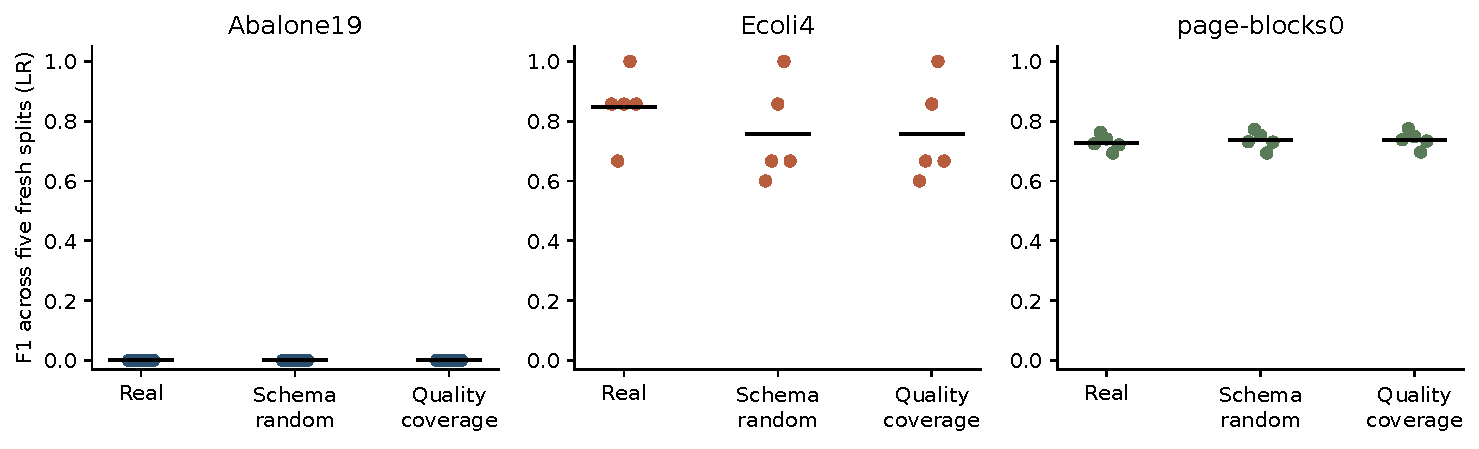
\includegraphics[width=\linewidth]{figures/repeated-f1.pdf}
\caption{Every fresh-split logistic F1 value; black bars show five-split means. Real-only and hybrid regimes are distinct. The page-blocks0 pool generator is ROS.}\label{fig:repeated}\end{figure}
Split-wise paired differences use identical evaluation records. Pure TSTR on offline minority-only pools is unavailable, never renamed hybrid augmentation.
